\section{System Design}
\label{sec:design}
AgentWorkShop is designed for industrial tasks whose agents, production
contexts, interfaces, and process signals vary between deployments. Its
architecture organizes these variations around shared task and operation
services, checks each proposed operation against the active production
context before device routing, and retains route-specific evidence that
distinguishes a command receipt from a measured process response.

\subsection{Design Rationale and Requirements}
\label{sec:principles}
Five requirements---scene variability, harness variability, operation
authority, outcome observability, and extensibility---organize six design
rules (D1--D6). These are deployment constraints drawn from the target
workflows. D1 stores scene settings as versioned data;
D2 provides registered harness, tool, and driver interfaces; D3 separates
proposal from execution; D4 treats the tool catalog as discovery rather than
permission; D5 routes actuator writes through the common DCW admission point;
and D6 retains evidence by operation.

The requirements trace to implementation as follows.
Scene variability maps to D1, scene blueprints, and context resolution;
harness variability and extensibility map to D2, the registered harness and
driver interfaces; operation authority maps to D3--D5, the shared dispatcher,
grants, bindings, and write admission; outcome observability maps to D6,
route-specific receipts, and observations. R13 exercises two scene-specific
protocol and data paths; R20 exercises the configured task-to-device path
through one registered harness, synthetic approvals, and route-specific
records. Section~\ref{sec:eval} reports the experimental scope and evidence
limits. AgentWorkShop supplies task and operation services; agent strategy
and independent process protection remain outside this design.

\subsection{Layered Architecture}
\label{sec:layers}
\label{sec:arch}
Fig.~\ref{fig:arch} maps the reference implementation onto six bands and
their route-specific evidence records. The access band exposes command-line,
web, SDK, REST, MCP, and A2A entry surfaces. Task and chat routes enter the
collaboration band, which contains workspaces, channels, task queues, shared
memory, mailboxes, task templates, and harness adapters. A direct REST
tool-invocation route can call the shared operation dispatcher without
creating a task or invoking a harness; MCP also includes separate management
and task operations. The governance band projects an operation catalog and
checks each invocation. The context band assembles bound-line and active-run
information for prompt grounding, while operation handlers resolve the live
state relevant to their route. The service band provides acquisition, write
control, analysis, retrieval, and optional model services. The field-I/O band
resolves semantic nodes to built-in or plugin drivers for a plant or
simulator.

Each band has a distinct responsibility. Task/chat routes enter the task
runtime; direct operation routes enter the dispatcher; and both use shared
operation checks where applicable. A harness adapter supplies
agent-specific interaction on task paths, semantic nodes hide protocol
details from operations, and the driver registry provides the device-facing
extension point. Owning services retain task, command, observation, and
version records separately and link them to available actor and production
context. No single status conflates these outcomes.

\subsection{Cross-Module Execution Flow}
\label{sec:executionflow}
Fig.~\ref{fig:runtime} summarizes a task turn from entry through operation
execution, with route-specific evidence retained by owning services. Registered
harness adapters receive a scoped tool catalog during setup and supported
registry refreshes; the runtime assembles prompt-time production context for
each agent turn. This context is grounding information, not a task-pinned
transaction. For each returned tool call, the shared dispatcher rechecks
invocation scope and channel policy and, for industrial operations, current
grant and binding conditions before handler selection. The selected handler
then applies route-specific guards, active-run checks, approval
revalidation, and device-I/O steps as applicable. Command receipts and later
process observations remain distinct records.

For an industrial operation $u$ by agent $a$ in channel $c$, define the
shared dispatch condition as
\begin{equation}
\mathcal{A}(a,c,u)=S(a,c,u)\land P(c,u)\land G(a,u)\land B(a,u),
\label{eq:dispatch-contract}
\end{equation}
where $S$, $P$, $G$, and $B$ denote invocation scope, current channel policy,
runtime grant, and agent binding/resource ownership. Scope and channel policy
are checked for every host-tool call. The grant check applies to industrial
tools except the explicit grant-exempt set; the binding/resource check applies
when the operation declares resource references. A declared no-reference
operation omits that term. Thus, the conjunction contains the checks selected
by the operation's dispatch declaration, and each included check must pass
before handler selection. The policy term includes channel tool selection,
profile, and duty-separation checks where configured. This condition is
necessary for handler selection, not sufficient for actuation: the selected
route applies its own guards and approval, then rechecks authority and
applicable limits before dispatch.

Fig.~\ref{fig:execution} gives reference pseudocode for the registered-harness
task path, not one literal orchestrator function. Direct REST tool invocation
bypasses the task runtime and harness but enters the same shared dispatcher.
Route-specific timing, approval, and evidence rules are detailed in
Section~\ref{sec:modules}.

\begin{figure*}[!t]
\centering
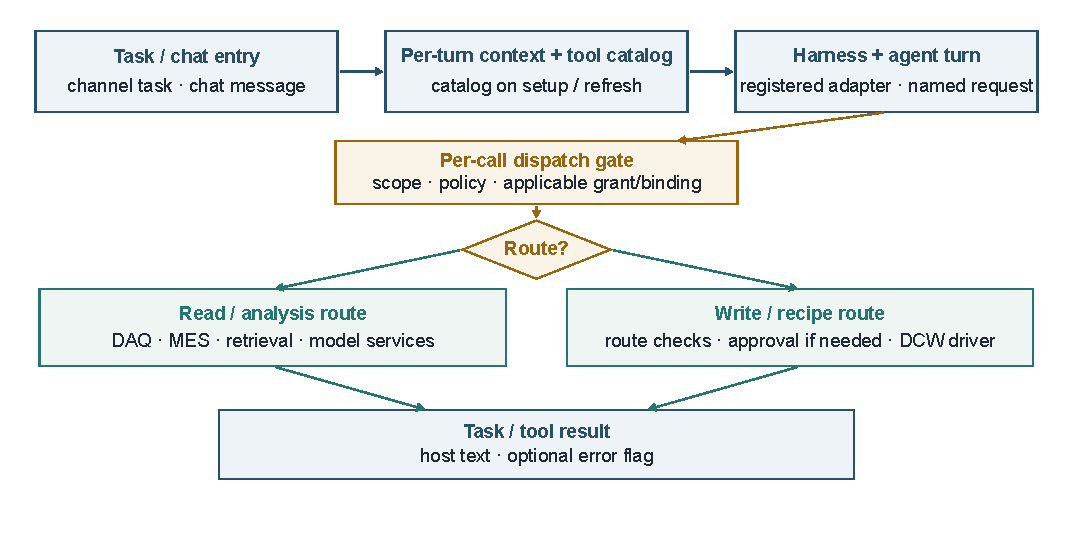
\includegraphics[width=\textwidth]{resources/fig-runtime-2026-9pt.pdf}
\caption{Registered-harness task execution in AgentWorkShop. The direct
REST tool-invocation route is outside this flow and enters the shared dispatcher
without a task or harness. The registered harness
uses a scoped catalog provisioned at setup and supported registry refreshes;
the runtime assembles prompt context per agent turn. The dispatcher checks
each returned call for scope, channel policy, and applicable grant and binding
conditions before handler selection. Route handlers resolve active-run and
approval-dependent state as applicable. The shared tool result contains host
text and an optional error flag; route records remain with owning services.
Prompt context is not a transactional authorization token. Dispatch-gate
errors return before handler execution, whereas route handlers may read state
before refusing a write. Durable denial auditing is selective. Receipts and
later observations remain distinct.}
\label{fig:runtime}
\end{figure*}

\begin{figure}[!t]
\centering
\begin{algorithmic}[1]
\Require task $q$, channel $c$, bound agent $a$, registered scoped catalog $T$
\Ensure task result; any retained evidence remains with its owning service
\State $x_t \gets \Call{ResolvePromptContext}{c,q}$
\State $m \gets \Call{RetrieveMemory}{q}$
\State $p \gets \Call{AssemblePrompt}{q,x_t,m}$
\State $h \gets \Call{InvokeRegisteredHarness}{a,p,T}$
\ForAll{tool request $u$ returned by $h$}
  \State $g \gets \Call{CheckScopeAndChannelPolicy}{a,c,u}$
  \If{\textbf{not} $g$}
    \State \Call{EmitToolErrorToHarness}{h,u}; \textbf{continue}
  \EndIf
  \If{$u$ is an industrial operation}
    \State $v \gets \Call{CheckGrantBindingOwnership}{a,u}$
    \If{\textbf{not} $v$}
      \State \Call{EmitToolErrorToHarness}{h,u}; \textbf{continue}
    \EndIf
  \EndIf
  \State $k \gets \Call{SelectHandler}{u}$
  \State $r \gets \Call{ExecuteRouteHandler}{k,a,c,u}$
  \Comment{handler resolves live state and may persist route-specific records}
  \State \Call{EmitDeclaredToolResultToHarness}{h,r}
\EndFor
\State \Return task state and tool results
\end{algorithmic}
\caption{Reference pseudocode for the registered-harness task path.
Direct operation invocation is not shown. Evidence persistence is
route-specific and remains with the owning service; the shared tool result
does not carry a generic evidence envelope.}
\label{fig:execution}
\end{figure}
